\section{Theorie}
\label{sec:Theorie}

\subsection{Die Erzeugung von Röntgenstrahlen}
Röntgenstrahlen werden hier mithilfe einer Glühkathode in einer evakuierten Röhre
erzeugt. Die Elektronen werden mithilfe des glühelektrischen Effektes emittiert und
durch ein elektrisches Feld auf eine Anode beschleunigt. Wenn die Elektronen die
Anode erreichen, entsteht Röntgenstrahlung. Diese wird aus zwei Quellen erzeugt,
aus dem kontinuierlichen Bremsspektrum und der charakteristischen Röntgenstrahlung
des Anodenmaterials.
\subsubsection{Das Bremsspektrum}
Das Bremsspektrum entsteht hierbei durch die Abbremsung des Elektrons im
Coulombfeld des Atomkerns. Dabei wird ein Photon ausgesandt, welches genau die
Energie besitzt, die das Elektron durch das Abbremsen verloren hat. Weil das
Elektron einen beliebigen Anteil seiner kinetischen Energie verlieren kann, ist
das Bremsspektrum kontinuierlich. Als maximale Obergrenze für den Energieverlust
ergibt sich die Wellenlänge
\begin{equation*}
  \lambda_{min} = \frac{h \cdot c}{e_0 U}.
\end{equation*}
Hierbei wird das Elektron vollständig abgebremst und seine kinetische Energie in
Strahlungsenergie umgesetzt.
\subsubsection{Das charakteristische Spektrum}
Wenn die Elektronen auf das Anodenmaterial treffen, werden Anodenatome ionisiert.
Dabei entstehen Lücken in den inneren Schalen der Atome. In diese Lücken können
Elektronen mit höheren Energien zurückfallen, was zu einer Energieabgabe in Form
von ausgesandten Photonen führt. Die abgegebene Energie entspricht genau der
Energiedifferenz zwischen den Schalen:
\begin{equation}
  h \nu = E_m - E_n.
  \label{eqn:absorptionskantentheorie}
\end{equation}
Aufgrund dieser von dem Anodenmaterial abhängigen Differenzen ergibt sich ein
diskretes, für das Material charakteristisches Spektrum. Dieses weist scharfe
Absorptionskanten auf, welche mit $K_{\alpha}, K_{\beta}, L_{\alpha}, ...$
bezeichnet werden. Hierbei steht das $K, L, ...$ für die Schale, auf der die
Übergänge enden und $\alpha, \beta, ...$ für den Ursprung des Elektrons.
Aufgrund der Abschirmung der Hüllenelektronen und der Wechselwirkung der
Elektronen verringert sich die Coulomb-Anziehung auf das äußere Elektron.
Daher ergibt sich für die Bindungsenergie eines Elektrons auf der $n$-ten
Schale:
\begin{equation}
  E_n = -R_{\infty} z_{eff}^2 \cdot \frac{1}{n^2}.
  \label{eqn:bindungsenergietheorie}
\end{equation}
Hierbei bezeichnet $R_{\infty} = 13.6 \si{\electronvolt}$ die Rydbergenergie,
$z_{eff} = z - \sigma$ die effektive Kernladung und $\sigma$ die
Abschirmkonstante. Konkret für die $K_{\alpha}$-Kante ergibt sich nach
\eqref{eqn:bindungsenergietheorie} die Energie $E_{K_\alpha}$:
\begin{equation}
  E_{K_\alpha} = R_{\infty} (z - \sigma_1)^2 \cdot \frac{1}{1^2} - R_{\infty} (z - \sigma_2)^2 \cdot \frac{1}{2^2}.
  \label{eqn:energiekalphatheorie}
\end{equation}
Aufgrund der inhomogenen Energieverteilung der äußeren Elektronen, welche durch
den Bahndrehimpuls und den Elektronenspin verursacht wird, ist jede der
charakteristischen Absorptionskanten in mehrere nebeneinander liegende Kanten
aufgteilt. Dies wird als Feinstruktur bezeichnet. Die Energien der einzelnen
Linien lassen sich nach der Sommerfeldschen Feinstrukturformel berechnen:
\begin{equation}
  E_{n,j} = -R_{\infty} \left( z_{eff,1}^2 \cdot \frac{1}{n^2} + \alpha^2 z_{eff,2}^4 \cdot \frac{1}{n^3} \left(  \frac{1}{j + \frac{1}{2}} - \frac{3}{4n} \right) \right).
  \label{eqn:sommerfeldtheorie}
\end{equation}
$\alpha$ bezeichnet hier die Sommerfeldsche Feinstrukturkonstante, $n$ die
Hauptquantenzahl und $j$ den Gesamtdrehimpuls.
Die Abschirmkonstante $\sigma_{K, abs}$ für Elektronen aus der $K$-Schale mit
der Hauptquantenzahl $n = 1$ ergibt sich dann nach \eqref{eqn:sommerfeldtheorie}:
\begin{equation}
  \sigma_K = Z - \sqrt{\frac{E_K}{R_\infty} - \frac{\alpha^2 Z^4}{4}}.
  \label{abschirmktheorie}
\end{equation}
Aufgrund der Komplexität der Bestimmung der Abschirmkonstante $\sigma_L$ wird durch
die Bestimmung der Differenz $\Delta E_L = E_{L_{II}} - E_{L_{III}}$ zwischen
zwei $L$-Kanten vereinfacht. Die $L_{I}$- sowie $L_{II}$-Kante kann in diesem
Versuch nicht gemessen werden. Daher ergibt sich für $\sigma_L$:
\begin{equation}
  \sigma_L = z - \left( \frac{4}{\alpha} \sqrt{\frac{\Delta E_L}{R_{\infty}}} - \frac{5 \Delta E_L}{R_{\infty}} \right)^{\frac{1}{2}} \left( 1 + \frac{19}{32} \alpha^2 \frac{\Delta E_L}{R_{\infty}} \right)^{\frac{1}{2}}
  \label{eqn:sigmaktheorie}
\end{equation}
Hierbei bezeichnet $z$ die Ordnungszahl.
Nach dem Moseley'schen Gesetz ist die Absorptionsenergie $E_K$ proportional zum Quadrat der Ordnungszahl $z$ des Absorbermaterials.
    Es gilt
    \begin{equation}
        E_K = R h (z - \sigma)^2
        \label{eqn:Moseley}
    \end{equation}
Um die Abschirmkonstanten $\sigma_1$, $\sigma_2$ und $\sigma_3$ für Kupfer
abschätzen zu können, werden folgende Gleichungen für die Emissionsenergien der
$K_\alpha$- sowie der $K_\beta$-Kante verwendet:
\begin{align}
  E_{K, abs}    & = R_{\infty} (z - \sigma_1)^2 \\
  E_{K, \alpha} & = R_{\infty} \left( \frac{1}{n} \right)^2 \cdot (z - \sigma_1)^2 - R_{\infty} \left( \frac{1}{m}\right)^2 \cdot (z - \sigma_2)^2 \\
  E_{K, \beta}  & = R_{\infty} \left( \frac{1}{n}\right)^2 \cdot (z - \sigma_1)^2 - R_{\infty} \left( \frac{1}{l} \right)^ \cdot (z - \sigma_3)^2 .
  \label{eqn:8}
\end{align}
Die Abschätzung gilt mit $n=1$, $m=2$ sowie $l=3$. Hierbei wurde der
Drehimpulsbeitrag vernachlässigt.

\subsection{Die Absorption der Röntgenstrahlung}
Bei Energien geringer als $1 \si{\mega\electronvolt}$ läuft die Absorption
hauptsächlich durch den Photoelektrischen Effekt und den Compton-Effekt ab.
Bei dem Auftreffen der Elektronen auf das Absorbermaterial nimmt der
Absorptionskoeffizient mit zunehmender Energie ab, er ist also antiproportional.
Wenn die Photonenenergie jedoch gerade größer ist als die Bindungsenergie eines
Elektrons aus einer inneren Schale steigt der Absorptionskoeffizient stark an.
Daher liegen die Absorptionskanten nach \eqref{eqn:absorptionskantentheorie} mit
$n = \infty$ gerade bei der Bindungsenergie des Elektrons. Diese Kanten sind in
folgender Abbildung dargestellt.
\begin{figure}[H]
  \centering
  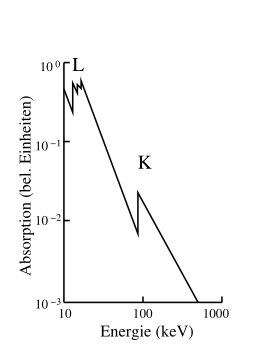
\includegraphics[scale=0.5]{"content/absorptionskanten.png"}
  \caption{Die Energie aufgetragen gegen die Größe der Absorptionskonstanten.}
  \label{fig:absorptionskanten}
\end{figure}
\noindent

\subsection{Die Braggsche Reflexion}
Um die Wellenlänge $\lambda$ der emittierten Röntgenstrahlung zu untersuchen,
kann die Braggsche Reflexion verwendet werden. Hierfür wird die Röntgenstrahlung
auf ein dreidimensionales Gitter treffen gelassen, was zu einer Beugung der Röntgenquanten
an den einzelnen Atomen des Gitters führt.  Bei dem Glanwinkel $\Theta$ interferieren
die gebeugten Röntgenquanten konstruktiv. Aus dem Glanzwinkel lässt sich dann
nach der Braggschen Bedingung die Wellenlänge bestimmen:
\begin{equation}
  2 d \sin \Theta = n \lambda.
  \label{eqn:braggtheorie}
\end{equation}
Hierbei bezeichnet $d$ die Gitterkonstante und $n$ die Beugungsordnung. Der
Sachverhalt ist in folgender Abbildung schematisch dargestellt.
\begin{figure}[H]
  \centering
  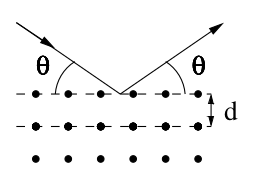
\includegraphics[scale=0.5]{"content/bragg.png"}
  \caption{Schematische Darstellung der Braggschen Reflexion.}
  \label{fig:braggtheorie}
\end{figure}
